%% The first command in your LaTeX source must be the \documentclass command.
\documentclass[acmtog]{acmart}
\usepackage[english,ngerman]{babel}
\usepackage[utf8]{inputenc} 
\usepackage{csquotes}

%% \BibTeX command to typeset BibTeX logo in the docs
\AtBeginDocument{%
  \providecommand\BibTeX{{%
    \normalfont B\kern-0.5em{\scshape i\kern-0.25em b}\kern-0.8em\TeX}}}
    
\copyrightyear{2024}
\acmYear{2024}
\citestyle{acmauthoryear}

\usepackage[figurename=Fig.]{caption}
\usepackage{csquotes}
\setcopyright{none}
\makeatletter
\renewcommand{\fnum@figure}{Abb. \thefigure}
\makeatother
\addto\captionsngerman{\renewcommand{\figurename}{Abb.}}
\settopmatter{printacmref=false} % Removes citation information below abstract
\renewcommand\footnotetextcopyrightpermission[1]{} % removes footnote with conference information in first column

%%
%% end of the preamble, start of the body of the document source.
\begin{document}

%%
%% The "title" command has an optional parameter,
%% allowing the author to define a "short title" to be used in page headers.
\title{Enterprise Architektur-Muster}

%%
%% The "author" command and its associated commands are used to define
%% the authors and their affiliations.
%% Of note is the shared affiliation of the first two authors, and the
%% "authornote" and "authornotemark" commands
%% used to denote shared contribution to the research.
\author{Julian Bruder}
\authornote{Alle Studierenden trugen zu gleichen Teilen zu dieser Arbeit bei.}
\author{Abdellah Filali}
\authornotemark[1]
\author{Luca Franke}
\authornotemark[1]
\affiliation{%
  \institution{Hochschule für Technik, Wirtschaft und Kultur Leipzig (HTWK Leipzig)}
  \streetaddress{Karl-Liebknecht-Str. 132}
  \city{Leipzig}
  %\state{Ohio}
  \country{Deutschland}
  \postcode{04277}
}
%%
%% By default, the full list of authors will be used in the page
%% headers. Often, this list is too long, and will overlap
%% other information printed in the page headers. This command allows
%% the author to define a more concise list
%% of authors names for this purpose.
\renewcommand{\shortauthors}{Bruder, Filali, Franke}

%%
%% The abstract is a short summary of the work to be presented in the
%% article.
\begin{abstract}
Blah \ldots
\end{abstract}

\maketitle

\section{Einleitung}
% (Beschreibung von Kontext, Problemen, Anforderungen und Zielen)
Blah \ldots

\section{Grundlagen von Enterprise-Architekturen}
Blah \ldots

\section{Klassische Enterprise-Architekturen}
Im folgenden Abschnitt werden klassische Architektur-Patterns vorgestellt. Dabei liegt der Fokus auf der monolithischen 
Architektur und der geschichteten (Layered) Architektur.

\subsection{Layered}
Das Layered Architektur-Pattern, auch bekannt als n-Tier-Archite
ktur-Pattern, gehört zu den am häufigsten verwendeten Architekturen. Laut \cite{layered}[S. 1] 
spiegelte diese Achitektur sowohl die Struktur der IT-Kommunikation als auch die organisatorische Struktur vieler Unternehmen wider,
was es zur bevorzugten Wahl für die meisten geschäftlichen Anwendungsarchitekturen machte. 

In dieser Architektur gibt es eine beliebige Anzahl von Schichten, die in zunehmenden Ebenen 
der Abstraktion und vertikal angeordnet sind (Siehe Abb. ~\ref{fig:layered}). 
Jede Schicht darf die Dienste der unmittelbar darunterliegenden Schicht nutzen.\cite{layered3}[S. 3]

Ein wichtige Eigenschaft der Layered Architecture ist der die Trennung der Zuständigkeiten 
(Englisch \textit{Separation of concerns}). Komponenten mit unterschiedlichen Aufgaben sollten 
auf verschiedene Schichten verteilt werden, sodass die Komponenten einer Schicht jeweils für 
eine klar definierte, gemeinsame Aufgabe zuständig sind. \cite {layered2}[S. 34]

Obwohl diese Architektur keine feste Anzahl an Schichten vorschreibt, 
bestehen die Layered Architectures meistens aus 3 Schichten \cite {layered2}:
\begin{itemize}
\item Presentations-Layer: Verantwortlich für die Interaktion mit dem Benutzer über die Benutzeroberfläche (UI). 
  Sie verarbeitet Benutzeranfragen und leitet diese an die Business-Layer weiter.
\item Busness-Layer: Zuständig für die Verarbeidung von Geschäftslogik und Regeln, die Weiteleitung von daten zwischen 
  die Presentation-Layer und die Data-Layer.
\item Data-Layer: Verantwortlich für die Interaktion mit Datenspeichern, wie beispielsweise Datenbanken,
  und die Kommunikation mit der Business-Layer, um Daten bereitzustellen oder die Ergebnisse entweder an die Presentation-Layer
  oder zurück an den Datenspeicher zu übermitteln. Darüber hinaus ermöglicht diese Schicht verschiedene Operationen auf den Daten,
  einschließlich deren Validierung sowie der Umsetzung von Sicherheitsmaßnahmen.
\end{itemize}

\begin{figure}[h!]
    \centering
    \includegraphics[width=0.2\textwidth]{images/layer.pdf}
    \caption{Layered Architektur}
    \label{fig:layered}
\end{figure}

Ein weiteren relevanten Konzept sind die \texttt{Open/Closed} Layers. Dieses beschreibt wie die 
Komunikation zwischen den Schichten erfolgt. \cite{layered4}[S. 10]
Standardmäßig sind die Schichten auf Closed gesetzt. Das bedeutet, dass eine Anfrage, 
zwingend die direkt darunterliegende Schicht durchlaufen muss, um zur übernächsten Schicht zu gelangen \cite{layered}[S. 3].(Siehe Abb. ~\ref{fig:layered-request-flow})
In manchen Situationen finden Architekten nützlich die Verwendung von Open Layers. Diese ermöglichen 
es, dass Kommunikation zwischen Schichten direkt zwischen benachbarten Schichten erfolgt, ohne die 
Open Layer durchlaufen zu müssen  (Siehe Abb. ~\ref{fig:layered-request-flow}). \cite{layered4}[S. 10]

\begin{figure}[h!]
    \centering
    \includegraphics[width=0.3\textwidth]{images/layer2.pdf}
    \caption{Open/Close Layering}
    \label{fig:layered-request-flow}
\end{figure}


Die Implementierung dieser Architektur bietet eine Reihe von Vorteilen. Durch 
die Aufteilung des Systems in verschiedene Schichten wird eine unabhängige 
Entwicklung und Wartung der einzelnen Schichten ermöglicht \cite{layered2}[S. 35]. 
Ein weiterer Vorteil besteht darin, dass der Zugriff auf die Dienste zwischen den 
Schichten über Schnittstellen (Interfaces) erfolgt. Dadurch sind Entwickler nicht 
gezwungen, die interne Implementierung einer Schicht zu kennen, um die bereitgestellten 
Dienste nutzen zu können. \cite{layered4}[S. 11]
Aufgrund der losen Kopplung der Schichten ist es zudem möglich, neue Funktionalitäten
hinzuzufügen oder Änderungen durch die Einführung neuer Schichten bzw. die Modifikation 
bestehender Schichten vorzunehmen, ohne dabei umfangreiche Anpassungen am gesamten 
System vornehmen zu müssen \cite{layered2}[S. 35].
Allerdings führt die Nutzung dieser Architektur zu einer geringeren Performance, da für 
den Zugriff auf Dienste in unteren Schichten eine Kette von Anfrageweiterleitungen erforderlich ist \cite{layered4}[S. 11].

\subsection{Monolith}
Die monolithische Architektur ist ein Softwarearchitektur-Pattern, bei dem die gesamte Funktionen in 
einer einzigen Anwendung zusammengefasst wird. 
In der Vergangenheit wurde diese Architektur von großen Internetdiensten wie Netflix, 
Amazon und eBay genutzt.\cite{mono}[S. 466]
Alle Komponenten in einer solchen Architektur sind voneinander abhängig, sodass sie 
weder eigenständig laufen noch in manchen Fällen überhaupt nicht isoliert kompiliert werden können. \cite{mono3}

\begin{figure}[h!]
    \centering
    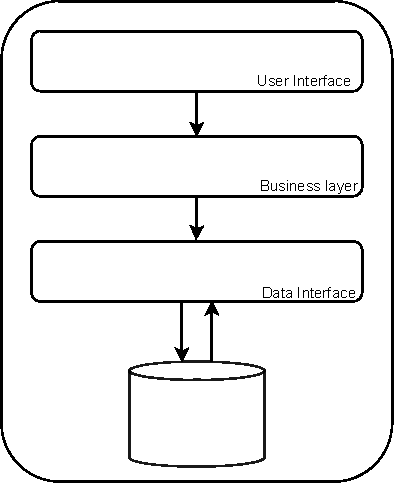
\includegraphics[width=0.2\textwidth]{images/mono.pdf}
    \caption{Monolith Architektur}
    \label{fig:mono}
\end{figure}

Einfachere Anwendungen, die diese Architektur nutzen, bieten einige Vorteile. 
Sie ermöglichen eine unkomplizierte Integration von querschnittlichen Belangen 
wie Logging oder Sicherheit, da alle Komponenten in derselben Anwendung laufen. 
Ein weiterer Vorteil ist die Reduzierung des Betriebsaufwands, da nur eine 
zentrale Anwendung deployed und betrieben werden muss. \cite{mono2}[S. 1]

Nachteile entstehen jedoch, wenn die Anwendung tatsächlich sehr groß und komplex 
wird. In diesem Fall kann die Komplexität und Unübersichtlichkeit des Code-Bases 
die Weiterentwicklung erschweren und Bugfixes behindern. \cite{mono}[S. 466]

Große Unternehmen wie Amazon und Netflix versuchen, von Microservices 
zu profitieren. Allerdings ist die Migration zu Microservices nicht immer 
die beste Wahl. So war es beispielsweise bei Amazon Prime Video, wo die Migration
rückgängig gemacht wurde und man zum Monolithen zurückkehrte. \cite{modular-mono2}[S. 10]
In Rahmen von solchen Migrationen die modulare Monolith-Architektur wurde immer populärer.
Diese kombiniert die Einfachheit der Monolithen Architektur mit den 
Vorteile der Microservice-Architektur, was einen Mittelweg zwischen 
den beiden Architekturen darstellt. \cite{modular-mono2}[S. 10 - S. 11]
Dieser Architektur wird erreicht, indem Domain-Driven Design auf eine
 traditionelle monolitische Architektur angewendet wird. Dadurch wird eine 
 große Domäne in mehrere isolierte Module unterteilt, was das Aufteilen 
 eines großen Teams in mehrere kleinere Teams ermöglicht. \cite{modular-mono1}[S. 49]
 Außerdem besteht die Möglichkeit, die Architektur zu einem 
späteren Zeitpunkt in eine Microservices-Architektur zu 
überführen, was eine flexiblere und effizientere Alternative darstellt
als eine direkte Migration \cite{modular-mono1}[S. 11].

\begin{figure}[h!]
    \centering
    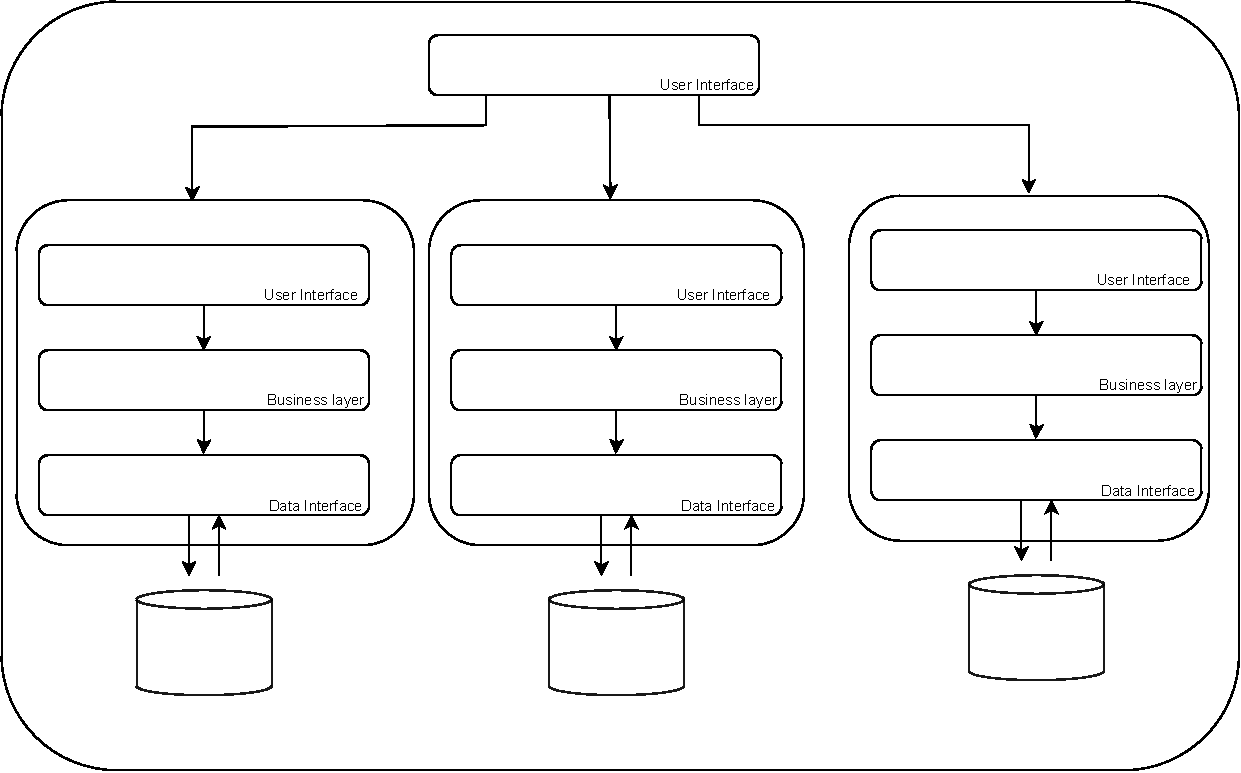
\includegraphics[width=0.5\textwidth]{images/mono-modular.pdf}
    \caption{Modular Monolith Architektur}
    \label{fig:modular-mono}
\end{figure}

Laut \cite{modular-mono2} die Haupteigenschaften von dieser Architektur sind:
\begin{itemize}
  \item Segregation der Module: Jedes Modul besitzt seine eigenen Schichten mit klaren Grenzen und ist unabhängig
    Die Komunikation erfolgt über API und oft asynchrone.
  \item Modularität mit losem Koppelung und hoher Kohäsion: Module sind lose gekoppelt aber mit hoche interne Kohäsionz. 
  \item Vereinheitlichtes Datenbankschema: Alle Module interagieren mit einem einzigen Datenschema
  \item Monolithische Deploymentsstruktur: Alle Module laufen auf eine einzigen Virtuale Maschine (VM). Jedoch es besteht weiterhin 
    die Möglichkeit die Module in einzeln VMs.
  \item Vereinheitlichter Anwendungsprozess: Die Anwendung läuft als ein einzelner Prozess, wobei es keine strikten Grenzen für den Datenbesitz zwischen den Modulen gibt.
  \item Verbesserte Wartbarkeit und Skalierbarkeit: Im Vergleich zu traditionellen Monolithen fördern modulare Monolithen die Wartbarkeit und Skalierung, indem sie eine bessere Bewältigung zunehmender Komplexität und eine Erleichterung des Wachstums ermöglichen.
\end{itemize}


\section{Moderne Enterprise-Architekturen}

\subsection{Event-Driven Architecture}
Die Event-Driven Architecture wählt als Basis einen anderen Ausgangspunkt als die bisherigen Architekturmuster.
Während bei letzteren Komponenten Dienste bereitstellen, welche von anderen Komponenten explizit genutzt werden,
verhalten sich Dienst-bereitstellende Komponenten in der Event-Driven Architecture reaktiv,
werden also implizit von Dienst-konsumierenden Komponenten genutzt \cite{garlanShawImplizit}.
Ein System reagiert somit asynchron auf Zustandsänderungen, also Ereignisse in diesem System \cite{eda}.
Die in dieser Architektur minimalen Einheiten, welche Informationen einer Zustandsänderung kapseln, werden \textit{Events} genannt.
Die Idee der impliziten Behandlung von Ereignissen ist nicht neu und taucht erstmals 1994 im von Garlan und Shaw publizierten Papier
\textit{\enquote{An introduction to Software Architecture}} auf.

Betrachten wir im Folgenden die Basis-Bestandteile der Event-Driven Architecture:
\begin{itemize}
  \item Ereignis (englisch \textit{Event}): Kapselt Information einer Zustandsänderung eines Systems
  \item Produzent (englisch \textit{Producer}): Komponente, die Event erzeugt
  \item Herausgeber (englisch \textit{Publisher}): Komponente, die, von Produzenten erzeugte, Events publiziert
  \item Konsument (englisch \textit{Consumer}): Reagiert auf publizierte Events
  \item Vermittler (englisch \textit{Mediator}): Liegt zwischen Produzenten und Konsumenten - filtert Events und verteilt diese auf Konsumenten
  \item Event-Bus: Oft auch \textit{Event-Broker} genannt - bietet die Infrastruktur für die Gesamtheit der Vermittler
\end{itemize}
Abstrakt kann ein Event als ein Vertrag zwischen Produzenten und Konsumenten am Event-Bus betrachtet werden.
Der Konsument nutzt die Spezifikation des Events am Bus, der Produzent implementiert jene Spezifikation.
Abbildung \ref{fig:eda} stellt diesen Vertrag dar.

\begin{figure}[!h]
  \centering
  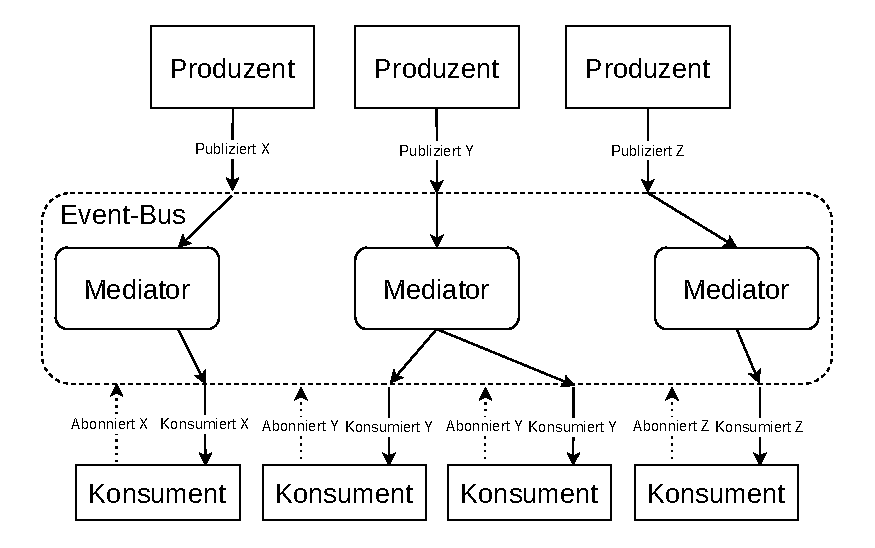
\includegraphics[width=\linewidth]{images/eda/eda.drawio}
  \caption{Vertrag zwischen Produzenten und Konsumenten am Event-Bus}
  \label{fig:eda}
\end{figure}

Durch den Vertrag weisen die Events am Event-Bus starke Kohäsion und somit lose Kopplung auf.
Diese lose Kopplung minimiert nicht nur kaskadierende Fehler, sondern ermöglicht agilen Entwickler-Teams durch klar abgegrenzte Features einfach definierbare Iterationen
- eine Menge von Events, deren Erzeugung und Konsumierung.

Weiter sind Events oft nah an dem, was Ereignisse in realen Prozessen sind, also domain-driven.
Gebündelt ermöglichen obige Punkte die kontinuierliche Auslieferung von Software in kurzen Intervallen.

Außerdem garantiert die asynchrone Behandlung von Ereignissen zusammen mit der loosen Kopplung maximale Skalierung.
Daher sind Event-Driven Architekturen besonders für datenintensive Echtzeit-Anwendungen wie IoT (Internet of Things) und Analytics geeignet \cite{iotEda}.

Die Agilität der Architektur kann weiter erhöht werden, indem der event-basierte Aspekt mit weiteren agilen Strukturen wie Microservices oder cloud-nativen Serverless-Functions kombiniert wird.
Die damit einhergehende Komplexität stellt teilweise hohe Anforderungen an die Entwickler.
Aufgrund der Asynchronität der Behandlung von Ereignissen ist die Testung des Systems meist schwer und die Fehlerbehandlung essentiell.
Mögliche Problemquellen schließen dabei unter anderem Event-Verlust, erhöhte Latenz und Inkonsistenz ein.
Die hohen Anforderungen an die Entwickler verlangen viel Vertrauen in jene, einer der zentralen Punkte des agilen Manifests \cite{agileManifesto}.
Insgesamt weist die Event-Driven Architecture also eine sehr hohe Agilität auf und ist damit besonders für moderne Software und ihre stetig wechselnden Anforderungen geeignet.

% TODO: Jetzt bestenfalls übergreifendes Beispiel

\section{Fallstudien und Praxisbeispiele}
Blah \ldots

\section{Diskussion}

\section{Zusammenfassung und Ausblick}
%(Überblick über die gesamte Arbeit, Rückführung auf Aussagen aus Kapitel 1 durchführen, offene Punkte als neue Forschungsfragen definieren)






\bibliographystyle{ACM-Reference-Format}
\bibliography{main}

\appendix

\section{Anhang 1}

\subsection{Übungsaufgaben}
Blah \ldots

\section{Anhang 2}
Blah \ldots

\end{document}
\endinput
